%----------------------------------------------------------------------------
\chapter{\SystemDesign}
%----------------------------------------------------------------------------

%----------------------------------------------------------------------------
\section{Követelmények}
%----------------------------------------------------------------------------






 

%----------------------------------------------------------------------------
\section{Rendszerterv}
%----------------------------------------------------------------------------








!!!ÁBRA HELYE!!!
Egy jel útja a régi hibrid rendszerben





!!!ÁBRA HELYE!!!
Egy jel útja az új teljesen digitális rendszerben

%----------------------------------------------------------------------------
\subsection{Martin Audio Wavefront Precision hangrendszer}
%----------------------------------------------------------------------------

\subsubsection{Martin Audio Display 2.3.4 b1 tervező szoftver}

Mielőtt bele kezdenénk a tervezési folyatba, fontos megemlíteni, hogy a szoftver 
eredetileg Intel alapú processzorokra lett tervezve és MatLab alapú. Ebből fakadóan
AMD processzorokon habár elidult a szoftver, de nem volt stabil és a számítások során
minden esetben összeomlott, és használtatalanul lassú volt. Személy szerint a saját gépem amivel dolgoztam
sajnos ilyen processzorral van szerelve ezért muszáj volt megoldást találni a problémára.
A Martin Audio hivatalos szoftveres támogatásához fordultam először, de sajnos nem tudtak segíteni.
Ezért a szoftver használatához
sok belefektetett óra olvasás után sikerült egy olyan MatLab CMD parancsot találnom, amivel
a szoftver elindul és használható. 
Miután rájöttem a probléma gyökerére, ezt megosztottam velük, hogy a jövőben másoknak ne kelljen
ezzel a problémával szembesülniük. 
A probléma az alábbi volt. Az új AMD processzorok másfajta utasításkészletet használnak. 
Ebből kifolyólag a MatLab alapú szoftver adta sima utasításokat nem tudta értelmezni a CPU.
A vezető szoftvermérnökkel való e-mail-es beszélgetésünk során megköszönte a probléma
megoldását, és nemsokkal a megoldásom megosztása után a hivatalos oldalra feltölttötték
az indító parancsfáljt. A kompatibilási probémát rögtön a script elején megoldottam,
mivel a következő parancs megadásával már használhatóvá válik a program: \texttt{set MKL\_DEBUG\_CPU\_TYPE=5} \newline
Ez a sor a program vezérlését AVX2-re állítja át, és mivel ezt az utasításkészletet ismeri az AMD processzor
is ezért a probléma már a múlté.
Az indító fájl további részei optimalizálások a számítások gyorsítására, és a párhuzamosításra AMD processzorokon.

\begin{lstlisting}[caption={A Display 2.3.4 b1 indító ".bat" scriptje AMD processzorokhoz}, label=batcode]
    @echo off
    set PATH=%PATH%;C:\Program Files\Martin Audio\Display2_3_4_b1\application
    set MKL_DEBUG_CPU_TYPE=5
    set options=optimoptions('ga','UseParallel',true,'UseVectorized',false)
    set options=optimoptions('gamultiobj','UseParallel',true,'UseVectorized',false)
    set options=optimoptions('paretosearch','UseParallel',true)
    set options=optimoptions('particleswarm','UseParallel',true,'UseVectorized',false)
    set options=optimoptions('patternsearch','UseParallel',true,'UseCompletePoll',true,'UseVectorized',false)
    set options=optimoptions('surrogateopt','UseParallel',true)
    set GPUAcceleration=on
    start "Martin Audio" Display2_3_4_b1.exe
    pause
\end{lstlisting}


\begin{figure}[!ht]
    \centering
    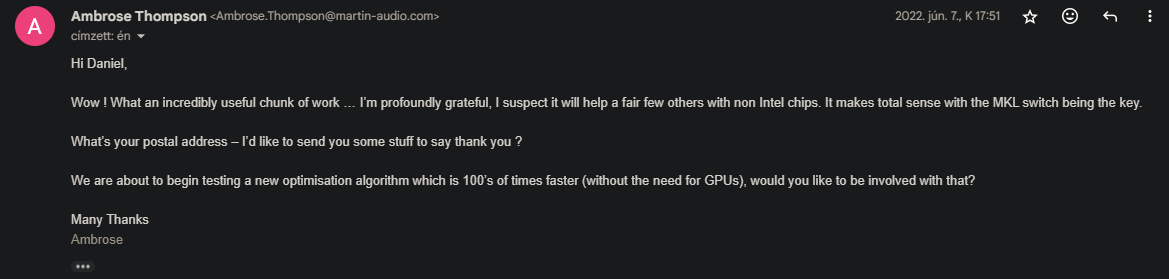
\includegraphics[width=150mm, keepaspectratio]{figures/ambrose_email.png}
    \caption{E-mail a Martin Audio vezető szoftvermérnökétől}
    \label{fig:ambrose_email}
\end{figure}


    
Most, hogy már a szoftver használható és teljes mértékben működőképes, kezdjük el a tervezést.
A modellezés során a budapesti Millenáris B csarnoka lesz a referencia helyszín. Két LineArray rendszert fogunk
tervezni, mivel a terem hosszúsága és a lefedettség növelése miatt szükségünk lesz Delay kiegészítésre a fő hangrendszerhez.








\subsubsection{Martin Audio VU-NET rendszer szoftver}



%----------------------------------------------------------------------------
\subsection{Allen \& Heath digitális keverőrendszer}
%----------------------------------------------------------------------------



%----------------------------------------------------------------------------
\subsection{Shure ULXD digitális vezeték nélküli mikrofonrendszer}
%----------------------------------------------------------------------------



%----------------------------------------------------------------------------
\subsection{Dante audio szerver}
%----------------------------------------------------------------------------



%----------------------------------------------------------------------------
\subsection{Dante hálózat kialakítása és optimalizálása}
%----------------------------------------------------------------------------

\subsubsection{Dante Controller: Hálózati mátrix}

Ezen a felületen tudjuk a hálózaton összekapcsolni a különböző hang vevőket és
adókat. Egy nagyobb rendszerben a konfigurálása rendkívül nagy odafigyelést és
precíziót igényel, pontosan tudnunk kell mit, hogyan és miért kötünk össze.

\subsubsection{Dante Controller: Eszköz nézet}

Mielőtt elkezdenénk konfigurálni az adott eszközt, fontos eldöntenünk, hogy
milyen módban szeretnénk használni.
Lehetőségünk van két fő mód közül választani, a redundáns és a
váltott mód közül. A redundant mód mint ahogy azt a neve is sugallja
redundáns kommunikációt valósít meg az eszközök között szoftveresen és
hardveresen egyaránt. Az összes Dante kártya a jelenlegi rendszerben gyárilag két RJ45-s
csatlakozóval rendelkezik. Jelen esetben ezt a módot választjuk az
üzembiztosság és a kritikus hibák minimalizálása miatt.
A másik lehetőség a váltott pedig eszközök láncolását
teszi egyszerűbbé. Amennyiben a rendundancia nem elsődleges szempont számunkra, nem kell
minden egyes eszköz mögé switch, hanem a másodlagos RJ45 port direktbe köti
az arra csatlakoztatott eszközt az elsődleges hálózatra. Így gyorsabban és
költséghatékonyabban tudjuk kiépíteni a hálózatot, azonban a redundancia lehetősége megszűnik. 

\subsubsection{IP kiosztás}

A rendszer képes automatikusan IP címeket osztani az egyes eszközöknek, 
így meggyorsítva a munkafolyamatot.
Azonban egy fixen előre megtervezett rendszernél praktikusabb és
üzembiztosabb megoldás, ha minden eszköznek manuálisan megadjuk a címét a
hálózaton. A tervezett rendszerben minden egyes eszköznek fix IP címet adtam,
hogy könnyen és logikusan átlátható legyen az előbb említett előnyökön kívül.
A címeket egy online is elérhető Excel táblázatban tároltam, hogy amennyiben szükség van rá
bármikor könnyen elérhető legyen. Ez a táblázat a cégnél dolgozó összes munkatárs számára látható,
aki a rendszerrel foglalkozik. Így amennyiben új eszköz kerül a hálózatra, vagy egy eszköz IP címét
valamilyen okból meg kell változtatni, egyszerűen elérhető a szükséges információ.


\begin{figure}[!ht]
\centering
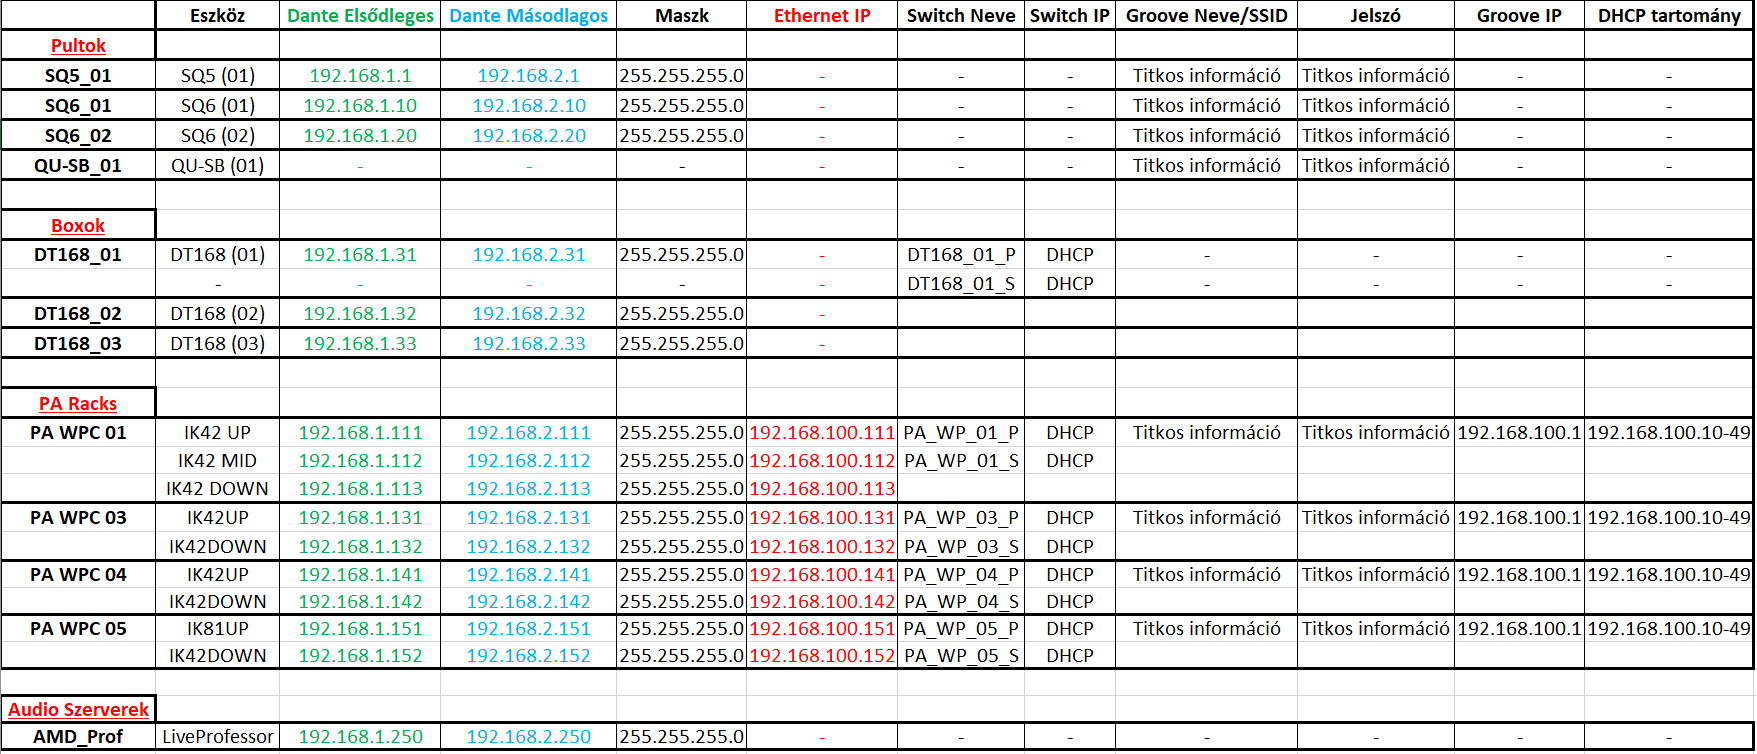
\includegraphics[width=150mm, keepaspectratio]{figures/dante_ips.png}
\caption{Dante eszközök IP címei a hálózaton}
\label{fig:dante_ips}
\end{figure}








\subsubsection{Dante Controller: Órajel nézet}

Meg kell adnunk az audio hálózatunk master órajelét, ehhez az órajelhez
szinkronizál a többi eszköz, az időszinkronizáció kulcsontosságú élőzenei
produkcióknál.



%----------------------------------------------------------------------------
\section{Rendszermérések és monitorozás}
%----------------------------------------------------------------------------




\subsection{Dante rendszer monitorozása}





\subsubsection{Dante Controller: Hálózati állapot nézet}





\subsubsection{Dante Controller: Események nézet}





%----------------------------------------------------------------------------
\subsection{Cardioid mélyláda rendszer mérése}
%----------------------------------------------------------------------------



%----------------------------------------------------------------------------
\subsection{Mélyláda és Line Array fázishelyesség}
%----------------------------------------------------------------------------



%----------------------------------------------------------------------------
\subsection{Rendszer hangnyomás szint és frekvencia átvitel mérése}
%----------------------------------------------------------------------------







